\documentclass{article}
% All LaTeX documents including
% tikz() output must use this
% package!
\usepackage{tikz}
\usepackage{multirow}
\usepackage{graphicx}
\usepackage[top=0.5cm, bottom=0.5cm, outer=0.5cm, inner=0.5cm, heightrounded,
  marginparwidth=0.5cm, marginparsep=0.2cm]{geometry}
\begin{document}
\begin{figure}[!h]
\centering
    \begin{tabular}{| l | *{3}{r} | c c c |}
      \hline
      \multirow{1}{*}Threads & gnparser & gbif-parser & biodiversity
      & \multicolumn{3}{c |}{Ratio} \\
      \cline{5-7}
      & & & & gn & gbif & bio \\
      \hline
      1  & 8178  & 6389  & 1111 & 1 & 0.78 & 0.14 \\
      2  & 14125 & 12638 & 1722 & 1 & 0.89 & 0.12 \\
      4  & 25125 & 21994 & 2556 & 1 & 0.88 & 0.10 \\
      8  & 33541 & 30972 & 2777 & 1 & 0.92 & 0.08 \\
      12 & 36369 & 31833 & 2527 & 1 & 0.88 & 0.07 \\
      \hline
    \end{tabular}
    % Created by tikzDevice version 0.9 on 2015-12-21 16:35:00
% !TEX encoding = UTF-8 Unicode
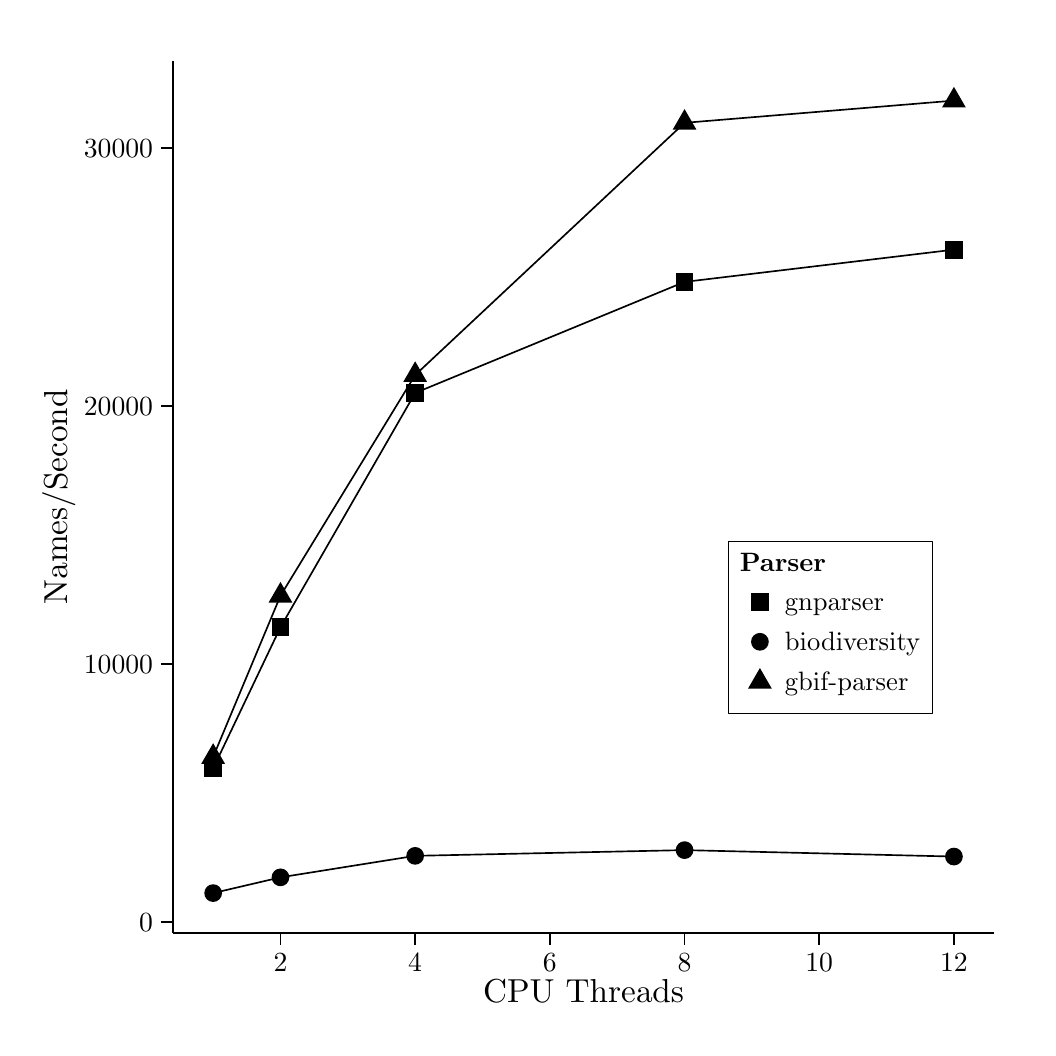
\begin{tikzpicture}[x=1pt,y=1pt]
\definecolor{fillColor}{RGB}{255,255,255}
\path[use as bounding box,fill=fillColor,fill opacity=0.00] (0,0) rectangle (361.35,361.35);
\begin{scope}
\path[clip] (  0.00,  0.00) rectangle (361.35,361.35);
\definecolor{drawColor}{RGB}{255,255,255}
\definecolor{fillColor}{RGB}{255,255,255}

\path[draw=drawColor,line width= 0.6pt,line join=round,line cap=round,fill=fillColor] (  0.00,  0.00) rectangle (361.35,361.35);
\end{scope}
\begin{scope}
\path[clip] ( 52.42, 34.31) rectangle (349.30,349.30);
\definecolor{fillColor}{RGB}{255,255,255}

\path[fill=fillColor] ( 52.42, 34.31) rectangle (349.30,349.30);
\definecolor{drawColor}{RGB}{255,255,255}

\path[draw=drawColor,line width= 0.6pt,line join=round] ( 52.42, 38.27) --
	(349.30, 38.27);

\path[draw=drawColor,line width= 0.6pt,line join=round] ( 52.42,131.48) --
	(349.30,131.48);

\path[draw=drawColor,line width= 0.6pt,line join=round] ( 52.42,224.69) --
	(349.30,224.69);

\path[draw=drawColor,line width= 0.6pt,line join=round] ( 52.42,317.90) --
	(349.30,317.90);

\path[draw=drawColor,line width= 0.6pt,line join=round] ( 91.35, 34.31) --
	( 91.35,349.30);

\path[draw=drawColor,line width= 0.6pt,line join=round] (140.02, 34.31) --
	(140.02,349.30);

\path[draw=drawColor,line width= 0.6pt,line join=round] (188.69, 34.31) --
	(188.69,349.30);

\path[draw=drawColor,line width= 0.6pt,line join=round] (237.36, 34.31) --
	(237.36,349.30);

\path[draw=drawColor,line width= 0.6pt,line join=round] (286.03, 34.31) --
	(286.03,349.30);

\path[draw=drawColor,line width= 0.6pt,line join=round] (334.70, 34.31) --
	(334.70,349.30);
\definecolor{drawColor}{RGB}{0,0,0}

\path[draw=drawColor,line width= 0.6pt,line join=round] ( 67.02, 48.63) --
	( 91.35, 54.32) --
	(140.02, 62.09) --
	(237.36, 64.16) --
	(334.70, 61.83);

\path[draw=drawColor,line width= 0.6pt,line join=round] ( 67.02, 97.82) --
	( 91.35,156.08) --
	(140.02,235.82) --
	(237.36,326.96) --
	(334.70,334.99);

\path[draw=drawColor,line width= 0.6pt,line join=round] ( 67.02, 93.68) --
	( 91.35,144.69) --
	(140.02,229.35) --
	(237.36,269.48) --
	(334.70,281.13);
\definecolor{fillColor}{RGB}{0,0,0}

\path[fill=fillColor] ( 63.82, 90.48) --
	( 70.22, 90.48) --
	( 70.22, 96.88) --
	( 63.82, 96.88) --
	cycle;

\path[fill=fillColor] ( 88.15,141.48) --
	( 94.55,141.48) --
	( 94.55,147.89) --
	( 88.15,147.89) --
	cycle;

\path[fill=fillColor] (136.82,226.15) --
	(143.22,226.15) --
	(143.22,232.55) --
	(136.82,232.55) --
	cycle;

\path[fill=fillColor] (234.16,266.28) --
	(240.56,266.28) --
	(240.56,272.68) --
	(234.16,272.68) --
	cycle;

\path[fill=fillColor] (331.50,277.93) --
	(337.90,277.93) --
	(337.90,284.33) --
	(331.50,284.33) --
	cycle;

\path[fill=fillColor] ( 67.02,102.80) --
	( 71.33, 95.33) --
	( 62.71, 95.33) --
	cycle;

\path[fill=fillColor] ( 91.35,161.06) --
	( 95.66,153.59) --
	( 87.04,153.59) --
	cycle;

\path[fill=fillColor] (140.02,240.80) --
	(144.33,233.33) --
	(135.71,233.33) --
	cycle;

\path[fill=fillColor] (237.36,331.94) --
	(241.67,324.47) --
	(233.05,324.47) --
	cycle;

\path[fill=fillColor] (334.70,339.96) --
	(339.01,332.50) --
	(330.39,332.50) --
	cycle;

\path[fill=fillColor] ( 67.02, 48.63) circle (  3.20);

\path[fill=fillColor] ( 91.35, 54.32) circle (  3.20);

\path[fill=fillColor] (140.02, 62.09) circle (  3.20);

\path[fill=fillColor] (237.36, 64.16) circle (  3.20);

\path[fill=fillColor] (334.70, 61.83) circle (  3.20);
\end{scope}
\begin{scope}
\path[clip] (  0.00,  0.00) rectangle (361.35,361.35);
\definecolor{drawColor}{RGB}{0,0,0}

\path[draw=drawColor,line width= 0.6pt,line join=round] ( 52.42, 34.31) --
	( 52.42,349.30);
\end{scope}
\begin{scope}
\path[clip] (  0.00,  0.00) rectangle (361.35,361.35);
\definecolor{drawColor}{RGB}{0,0,0}

\node[text=drawColor,anchor=base east,inner sep=0pt, outer sep=0pt, scale=  1.00] at ( 45.30, 34.83) {0};

\node[text=drawColor,anchor=base east,inner sep=0pt, outer sep=0pt, scale=  1.00] at ( 45.30,128.04) {10000};

\node[text=drawColor,anchor=base east,inner sep=0pt, outer sep=0pt, scale=  1.00] at ( 45.30,221.25) {20000};

\node[text=drawColor,anchor=base east,inner sep=0pt, outer sep=0pt, scale=  1.00] at ( 45.30,314.46) {30000};
\end{scope}
\begin{scope}
\path[clip] (  0.00,  0.00) rectangle (361.35,361.35);
\definecolor{drawColor}{RGB}{0,0,0}

\path[draw=drawColor,line width= 0.6pt,line join=round] ( 48.15, 38.27) --
	( 52.42, 38.27);

\path[draw=drawColor,line width= 0.6pt,line join=round] ( 48.15,131.48) --
	( 52.42,131.48);

\path[draw=drawColor,line width= 0.6pt,line join=round] ( 48.15,224.69) --
	( 52.42,224.69);

\path[draw=drawColor,line width= 0.6pt,line join=round] ( 48.15,317.90) --
	( 52.42,317.90);
\end{scope}
\begin{scope}
\path[clip] (  0.00,  0.00) rectangle (361.35,361.35);
\definecolor{drawColor}{RGB}{0,0,0}

\path[draw=drawColor,line width= 0.6pt,line join=round] ( 52.42, 34.31) --
	(349.30, 34.31);
\end{scope}
\begin{scope}
\path[clip] (  0.00,  0.00) rectangle (361.35,361.35);
\definecolor{drawColor}{RGB}{0,0,0}

\path[draw=drawColor,line width= 0.6pt,line join=round] ( 91.35, 30.04) --
	( 91.35, 34.31);

\path[draw=drawColor,line width= 0.6pt,line join=round] (140.02, 30.04) --
	(140.02, 34.31);

\path[draw=drawColor,line width= 0.6pt,line join=round] (188.69, 30.04) --
	(188.69, 34.31);

\path[draw=drawColor,line width= 0.6pt,line join=round] (237.36, 30.04) --
	(237.36, 34.31);

\path[draw=drawColor,line width= 0.6pt,line join=round] (286.03, 30.04) --
	(286.03, 34.31);

\path[draw=drawColor,line width= 0.6pt,line join=round] (334.70, 30.04) --
	(334.70, 34.31);
\end{scope}
\begin{scope}
\path[clip] (  0.00,  0.00) rectangle (361.35,361.35);
\definecolor{drawColor}{RGB}{0,0,0}

\node[text=drawColor,anchor=base,inner sep=0pt, outer sep=0pt, scale=  1.00] at ( 91.35, 20.31) {2};

\node[text=drawColor,anchor=base,inner sep=0pt, outer sep=0pt, scale=  1.00] at (140.02, 20.31) {4};

\node[text=drawColor,anchor=base,inner sep=0pt, outer sep=0pt, scale=  1.00] at (188.69, 20.31) {6};

\node[text=drawColor,anchor=base,inner sep=0pt, outer sep=0pt, scale=  1.00] at (237.36, 20.31) {8};

\node[text=drawColor,anchor=base,inner sep=0pt, outer sep=0pt, scale=  1.00] at (286.03, 20.31) {10};

\node[text=drawColor,anchor=base,inner sep=0pt, outer sep=0pt, scale=  1.00] at (334.70, 20.31) {12};
\end{scope}
\begin{scope}
\path[clip] (  0.00,  0.00) rectangle (361.35,361.35);
\definecolor{drawColor}{RGB}{0,0,0}

\node[text=drawColor,anchor=base,inner sep=0pt, outer sep=0pt, scale=  1.20] at (200.86,  9.03) {CPU Threads};
\end{scope}
\begin{scope}
\path[clip] (  0.00,  0.00) rectangle (361.35,361.35);
\definecolor{drawColor}{RGB}{0,0,0}

\node[text=drawColor,rotate= 90.00,anchor=base,inner sep=0pt, outer sep=0pt, scale=  1.20] at ( 14.29,191.81) {Names/Second};
\end{scope}
\begin{scope}
\path[clip] (  0.00,  0.00) rectangle (361.35,361.35);
\definecolor{drawColor}{RGB}{0,0,0}
\definecolor{fillColor}{RGB}{255,255,255}

\path[draw=drawColor,line width= 0.3pt,line join=round,line cap=round,fill=fillColor] (253.09,113.49) rectangle (326.76,175.63);
\end{scope}
\begin{scope}
\path[clip] (  0.00,  0.00) rectangle (361.35,361.35);
\definecolor{drawColor}{RGB}{0,0,0}

\node[text=drawColor,anchor=base west,inner sep=0pt, outer sep=0pt, scale=  0.96] at (257.36,164.73) {\bfseries Parser};
\end{scope}
\begin{scope}
\path[clip] (  0.00,  0.00) rectangle (361.35,361.35);
\definecolor{drawColor}{RGB}{255,255,255}
\definecolor{fillColor}{RGB}{255,255,255}

\path[draw=drawColor,line width= 0.6pt,line join=round,line cap=round,fill=fillColor] (257.36,146.67) rectangle (271.82,161.12);
\end{scope}
\begin{scope}
\path[clip] (  0.00,  0.00) rectangle (361.35,361.35);
\definecolor{fillColor}{RGB}{0,0,0}

\path[fill=fillColor] (261.39,150.69) --
	(267.79,150.69) --
	(267.79,157.09) --
	(261.39,157.09) --
	cycle;
\end{scope}
\begin{scope}
\path[clip] (  0.00,  0.00) rectangle (361.35,361.35);
\definecolor{drawColor}{RGB}{255,255,255}
\definecolor{fillColor}{RGB}{255,255,255}

\path[draw=drawColor,line width= 0.6pt,line join=round,line cap=round,fill=fillColor] (257.36,132.21) rectangle (271.82,146.67);
\end{scope}
\begin{scope}
\path[clip] (  0.00,  0.00) rectangle (361.35,361.35);
\definecolor{fillColor}{RGB}{0,0,0}

\path[fill=fillColor] (264.59,139.44) circle (  3.20);
\end{scope}
\begin{scope}
\path[clip] (  0.00,  0.00) rectangle (361.35,361.35);
\definecolor{drawColor}{RGB}{255,255,255}
\definecolor{fillColor}{RGB}{255,255,255}

\path[draw=drawColor,line width= 0.6pt,line join=round,line cap=round,fill=fillColor] (257.36,117.76) rectangle (271.82,132.21);
\end{scope}
\begin{scope}
\path[clip] (  0.00,  0.00) rectangle (361.35,361.35);
\definecolor{fillColor}{RGB}{0,0,0}

\path[fill=fillColor] (264.59,129.96) --
	(268.90,122.50) --
	(260.28,122.50) --
	cycle;
\end{scope}
\begin{scope}
\path[clip] (  0.00,  0.00) rectangle (361.35,361.35);
\definecolor{drawColor}{RGB}{0,0,0}

\node[text=drawColor,anchor=base west,inner sep=0pt, outer sep=0pt, scale=  0.96] at (273.62,150.59) {gnparser};
\end{scope}
\begin{scope}
\path[clip] (  0.00,  0.00) rectangle (361.35,361.35);
\definecolor{drawColor}{RGB}{0,0,0}

\node[text=drawColor,anchor=base west,inner sep=0pt, outer sep=0pt, scale=  0.96] at (273.62,136.13) {biodiversity};
\end{scope}
\begin{scope}
\path[clip] (  0.00,  0.00) rectangle (361.35,361.35);
\definecolor{drawColor}{RGB}{0,0,0}

\node[text=drawColor,anchor=base west,inner sep=0pt, outer sep=0pt, scale=  0.96] at (273.62,121.68) {gbif-parser};
\end{scope}
\end{tikzpicture}

\end{figure}
\end{document}
